% Yeban User Guide — Chapter 5: Recording and Audio Editing (English)
% T-DOC-001 chapter-by-chapter delivery, written ahead of the CH05 task.
% Sources: app.slint menus/callbacks, host.rs recording wiring, record_landing.rs,
% docs/manual/03-tracks-clips.md, cli.rs SHORTCUTS.

\chapter{Recording and Audio Editing}
\label{ch:recording-audio}

This chapter covers getting outside sound into a project: recording, importing,
placing audio clips on tracks, and basic trimming and fading. Recorded and imported
material goes into the project's asset pool and travels with it.

\section{Recording Flow and Input Monitoring}

\subsection{Open the record panel}

File $\to$ Record WAV in Real Time... opens the recording panel. It has an Arm switch,
input-device selection and an input test; the recording path uses the project's sample
rate (48 kHz by default). Transport keys are recording-aware: stopping ends the write
rather than quietly carrying on.

\screenshot{ch05-record-panel}{The recording panel with the Arm switch, input-device selection and level monitoring}

\subsection{Where recordings land}

After a successful stop, the bytes land in the project's asset pool with their real
decoded facts (frames, sample rate, channels, bit depth) and, when the wiring is
complete, an ``add clip'' operation is committed to the project — so the recording
appears on the timeline, not only as a WAV on disk. If the current assembly does not
wire the recording write face into the project, the app only writes to disk and does
not pretend a commit happened; that is existing headless/diagnostic behaviour.

\begin{figure}[htbp]
\centering
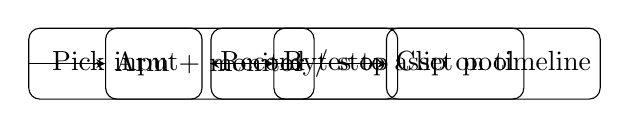
\begin{tikzpicture}[node distance=1.2cm, >=stealth,
    box/.style={draw, rounded corners, align=center, minimum width=2.2cm, minimum height=0.9cm}]
  \node[box] (a) {Pick input};
  \node[box, right of=a] (b) {Arm + monitor};
  \node[box, right of=b] (c) {Record / stop};
  \node[box, right of=c] (d) {Bytes to asset pool};
  \node[box, right of=d] (e) {Clip on timeline};
  \draw[->] (a)--(b); \draw[->] (b)--(c); \draw[->] (c)--(d); \draw[->] (d)--(e);
\end{tikzpicture}
\caption{Recording path: pick input $\to$ arm/monitor $\to$ record/stop $\to$ asset pool $\to$ timeline clip}
\label{fig:ch05-record-flow}
\end{figure}

\section{Audio Clip Trim, Fade In/Out and Crossfade}

\subsection{Import and place}

File $\to$ Import Audio File... reads audio into the project; Track $\to$ Place Latest
Imported Audio on Current Audio Track puts it on the current audio track's timeline.
The landing point follows the playhead and the selected track, so check both before
placing to avoid putting material on the wrong track or at the wrong position.

\subsection{Trim and fade}

Once placed, dragging a clip's left or right edge changes its time span: trimming
leading silence or trailing excess is the most common audio cleanup. A fade-in brings
the head up from silence; a fade-out lets the tail die away; a crossfade across the
overlap of two adjacent clips removes an abrupt seam.

The exact entry points for these operations (clip parameter area, context menu or
Edit menu) depend on the build you use; do not assume a control that is not present.
Fades change only the gain envelope, never the original bytes in the asset pool.

\screenshot{ch05-audio-clip-edges}{An audio clip with draggable left/right edges and fade handles labelled}

\subsection{Don't be misled by a "complete" message}

Stem export measures what was actually rendered and skipped. If every audio clip in a
stem was skipped, the receipt should give the clip-skip count and downgrade the
message rather than still saying merely ``stems complete''. Even when you see
``complete'', cross-check the counts in the receipt (Chapter 8).

\section{The Asset Pool and Audio Asset Management}

Bytes from recording and importing go into the project's asset pool, addressed by
content hash. The direct benefit is a self-contained project: copy the \texttt{.yeban}
file and the sounds it uses travel with the container, so opening it on another
machine does not turn it silent.

\screenshot{ch05-asset-pool}{The asset pool panel listing a project's audio assets and content hashes}

\section{Help Topic Mapping}

\begin{table}[htbp]
\centering
\caption{Sections of this chapter $\to$ in-app help anchors}
\label{tab:ch05-help}
\begin{tabular}{ll}
\hline
Section & Help topic \\
\hline
Record panel / input monitoring & \texttt{record-panel-input} \\
Where recordings land & \texttt{record-landing} \\
Import and place & \texttt{audio-import-place} \\
Trim and fade & \texttt{audio-trim-fade} \\
Don't be misled by ``complete'' & \texttt{audio-receipt-honesty} \\
Asset pool and audio assets & \texttt{audio-asset-pool} \\
\hline
\end{tabular}
\end{table}

\paragraph{What you will be able to do} Record and land a clip on the intended track, import and trim audio, add fades, and verify an export against the receipt.

\paragraph{Hands-on exercise} Create an audio track and put the playhead at 001.01.000; record two bars with Record WAV in Real Time... and stop, verifying the clip appears on the timeline; trim the leading silence and add a fade-out; import another file and place it on a second track with Place Latest Imported Audio...; finally export stems and compare the clip counts in the receipt.
